
% This is the "preamble" of the document. This is where the format options get set.
% Pro-tip: things following the % mark will not be compiled by LaTeX. I'll be using them extensively to explain things as we go.
% Note: not to scare you off of LaTeX, but it's normal to have problems. And ya girl has been having some. I've included the copyright info at the bottom of the document from the guy who wrote this package, because his documentation doesn't entirely match how it's actually used. So this is a combination of his working preamble along with my added commentary or explanation. 
%% 


\documentclass[stu,12pt,floatsintext]{apa7}
% Document class input explanation ________________
% LaTeX files need to start with the document class, so it knows what it's using
% - This file is using the apa7 document class, as it has a lot of the formatting built in
% There are two sets of brackets in LaTeX, for each command (the things that start with the slash \ )
% - The squiggle brackets {} are mandatory for executing the command
% - The square brackets [] are options for that command. There can be more than one set of square brackets for some commands
% Options used in this document (general note - for each of these, if you want to use the other options, swap it out in that spot in the square brackets):
% - stu: this sets the `document mode' as the "student paper" version. Other options are jou (journal), man (manuscript, for journal submission), and doc (a plain document)
% --- The student setting includes things like 'duedate', 'course', and 'professor' on the title page. If these aren't wanted/needed, use the 'man' setting. It also defaults to including the tables and figures at the end of the document. This can be changed by including the 'floatsintext' option, as I have for you. If the instructor wants those at the end, remove that from the square brackets.
% --- The manuscript setting is roughly what you would use to submit to a journal, so uses 'date' instead of 'duedate', and doesn't include the 'course' or 'professor' info. As with 'stu', it defaults to putting the tables and figures at the end rather than in text. The same option will bump those images in text.
% --- Journal ('jou') outputs something similar to a common journal format - double columned text and figurs in place. This can be fun, especially if you are sumbitting this as a writing sample in applications.
% --- Document ('doc') outputs single columned, single spaced text with figures in place. Another option for producing a more polished looking document as a writing sample.
% - 12pt: sets the font size to 12pt. Other options are 10pt or 11pt
% - floatsintext: makes it so tables and figures will appear in text rather than at the end. Unforunately, not having this option set breaks the whole document, and I haven't been able to figure out why. IT's GREAT WHEN THINGS WORK LIKE THEY'RE SUPPOSED TO.

\usepackage[american]{babel}

\usepackage{csquotes} % One of the things you learn about LaTeX is at some level, it's like magic. The references weren't printing as they should without this line, and the guy who wrote the package included it, so here it is. Because LaTeX reasons.
\usepackage[style=apa,sortcites=true,sorting=nyt,backend=biber]{biblatex}
% biblatex: loads the package that will handle the bibliographic info. Other option is natbib, which allows for more customization
% - style=apa: sets the reference format to use apa (albeit the 6th edition)
\DeclareLanguageMapping{american}{american-apa} % Gotta make sure we're patriotic up in here. Seriously, though, there can be local variants to how citations are handled, this sets it to the American idiosyncrasies 
\addbibresource{Spoofing Project.bib} % This is the companion file to the main one you're writing. It contains all of the bibliographic info for your references. It's a little bit of a pain to get used to, but once you do, it's the best. Especially if you recycle references between papers. You only have to get the pieces in the holes once.`
\addbibresource{bibliography.bib}

\usepackage[T1]{fontenc} 
\usepackage{mathptmx} % This is the Times New Roman font, which was the norm back in my day. If you'd like to use a different font, the options are laid out here: https://www.overleaf.com/learn/latex/Font_typefaces
% Alternately, you can comment out or delete these two commands and just use the Overleaf default font. So many choices!


% Title page stuff _____________________
\title{Approaches to Prevention and Detection of Malicious AIS Data} % The big, long version of the title for the title page
\shorttitle{AIS Spoofing} % The short title for the header
\author{Joey Simone}
\duedate{April 20, 2024}
% \date{January 17, 2024} The student version doesn't use the \date command, for whatever reason
\affiliation{California State University Maritime Academy}
\course{MT Capstone} % LaTeX gets annoyed (i.e., throws a grumble-error) if this is blank, so I put something here. However, if your instructor will mark you off for this being on the title page, you can leave this entry blank (delete the PSY 4321, but leave the command), and just make peace with the error that will happen. It won't break the document.
\professor{Dr. Bets McNie}  % Same situation as for the course info. Some instructors want this, some absolutely don't and will take off points. So do what you gotta.

\abstract{The Automatic Identification System, AIS, has been unchanged for many years. Vessels communicate in an enencrypted unsigned way, creating a threat vector for cybercrime, cyberwarfare, and cyberdiplomacy in the Maritime Environment. This paper reviews possible changes that could be made to AIS to increase the safety of mariners as well as protect the environment.}

%\keywords{APA style, demonstration} % If you need to have keywords for your paper, delete the % at the start of this line

\begin{document}
\maketitle % This tells LaTeX to make the title page

% \section{Introduction} This command is commented out, because I was taught it was redundant to have the paper's title and introduction together. If your instructor wants it to say "Introduction", delete the % at the start

The modernization of the Maritime Industry has included many lifesaving improvements to our navigation and communication equipment and protocols. The Automatic Identification System (AIS) has decades of service facilitating vessel communication and preventing collisions; the use of AIS Aids to Navigation (AIS AToNS) is very useful for establishing marks where it is impossible to rig a traditional buoy, or to temporarily mark a dangerous position while traditional marks are installed. The AIS, when given true information and interpreted by competent officers, has saved lives, and will save countless more. However, the advent of cyberwarfare jeopardizes the safety of mariners like us, and AIS has minimal security features for preventing attacks. A solution must be adopted which verifies a message’s sender’s identity, that the message has not been tampered with, and that the content of the message is genuine.

Since the Introduction is where references in papers first show up, let us incorporate some now. There are some intricacies to be aware of when using \LaTeX{} to write your paper (yes, there is a \LaTeX{} command to make it look fancy like that, because of course there is). Referencing something \textbf{in text} is done by dropping the name in text with the year followed in parentheses; lucky for us \LaTeX{} handles it with the right command, like  \textcite{Sample2024}. But maybe you want to just include it all at as a \textbf{parenthetical}? \LaTeX{} can do that as well \parencite{FullBook2021}. %For multi-author works \parencite[e.g.,]{Multiauthor2020}, the full author list will be included the first time. However, on subsequent reappearances of that reference, it will be shortened as APA intended \parencite{Multiauthor2020}.
For whatever reason, it does not seem like the multi-author work \parencite[e.g.,][]{Multiauthor2020} is working as it should, where it gives the full list the first time it is included in text, then truncates afterwards \parencite{Multiauthor2020}. I am not sure what is up with that, so the best advice I can offer you is to do write out the first instance yourself, then let \LaTeX{} handle the rest. It sucks, I know. Such is the nature of the \LaTeX{} beast, sometimes.

As a formatting note, the References page needs to start on a new page. This \textit{should be} handled automatically by \LaTeX{}, but it's still useful to know the format.

While I have your attention before diving into the sections, something that may slip by unnoticed is the \LaTeX{} quirk about quotation marks. If you were to include a quote using the regular quotation marks, "it will look like this." However, the \LaTeX{} specific way of doing it, that just gives it that little bit extra flair, is to use a double tick mark (on the tilde key up on the number row) to start the quote, and a double apostrophe to close it. That will make the quote ``look like this instead.'' They are ``fun little guys'' hugging your quote, instead of the "more bland marks" you get from the regular quotation marks.

To close out this section, I will finally talk about the contents of the Introduction. In these sorts of papers, think of the information process in the shape of an hourglass (stay with me, it'll make sense). The general idea is that you start at the broadest point, work your way into more and more specific, until you are at the point of this paper - the theory its testing and the hypothesis. Then you stay in that specific level of detail through the Methods and Results. The Discussion starts specific (i.e., what you did or did not find), then work your way back out to the broader meaning or implications. 

\section{Method}

\subsection{DELETE THIS SECTION - this is an informative section, not something to be included in your final paper.}

I have tried to include the most I've seen asked of students in these papers. You may not need to fill out all of these boxes, in which case you can just delete them. Along with this subsection.

Also, I have seen many different combinations of these boxes - e.g., in one of my papers, I had a ``participants and materials'' section followed by a ``procedure and measures,'' but cannot remember why it was written that way. Maybe it is what the journal wanted? Moral of the story here: go with what the person who is making the decision about the quality of your paper wants. If they want everything in its own little box, do it. If they want some boxes combined, do that.

Just make sure you delete or comment out this subsection!

\subsection{Participants}

Talk about the people who participated in your study. How many students, sourced from where, reimbursed how, ethics assured by what?

\subsection{Materials}

What materials were used in the course of this experiment? Try to walk the line between being overly specific (i.e., ``pens were standard Bic Clio Stic of medium thickness'') while still having enough detail someone else could read your paper and replicate what you used.

Sometimes it can be helpful to include the stimuli used in the experiment. For example, here is an example table (Table \ref{tab:table_words}) of words that were used in this hypothetical experiment. If you make use of the label command, \LaTeX{} will handle numbering things for you.

% There's lots of little components to the table. For the most part you can just copy it, or build your own with Overleaf's table wizard up top. 
% I'll mention that the & character separates items into different columns on a row, and the \\ ends that line. \hline generates a line that matches the width of the table.
\begin{table}
    \caption{Sample words from this hypothetical experiment.}
    \centering
    \begin{tabular}{cc} %The c's here indicate the columns will be centered
        \hline 
         First word & Second word \\
         \hline
         Yeet & Yoink \\
         Hot & Lit \\
         \hline
    \end{tabular}
    \label{tab:table_words}
\end{table}




\subsection{Measures}

This sets up what measure(s) you took during your experiment, including information about \textit{how} those measures were gathered. Was it with some form of worksheet? Was it collected electronically? If electronic, was it through a website or something like E-Prime? If a keyboard was used, were there any specifics about the keys used?

\subsection{Design}

This is typically used to describe the conditions of the experiment. Did everyone experience the same things throughout the experiment, or were there counterbalances, such as for item order exposure, condition order exposure, conditions on days, etc.? 

For undergrad research projects, lab instructors generally try to encourage students towards easier projects, as analyzing a 3 x 2 x 5 experiment is rough, no matter how far along the academic process you are. So I would expect to see something more along the lines of a 2 (experimental manipulation) x 2 (order counterbalance) design.


\subsection{Procedure}

From the time the participant starts the experiment to the time they leave, what did they experience? After informed consent was obtained, what did they do? Or, in some cases, what did you do to them? \textit{What did you do to them?} Make sure you highlight parts where things may deviate from the norm, such as in the debrief, needing to reveal to participants they hadn't been informed of the full nature of the experiment earlier as it would have impacted their ability to respond honestly or otherwise contaminated the data.



\section{Results}

Some instructors will want things broken down with the subheadings (e.g., `Descriptive Statistics') I have included, some will light your paper on fire if you \textit{do} include these. Always check with the assignment/rubric for what is wanted. Also, don't check my math on these, I am making all of the numbers up as we go, so it's almost certainly not going to hang together correctly.

I'll add this tip in here: since \LaTeX{} uses the percent symbol as the signal to comment out/hide what's typed after it in that line, what do you do if you need that symbol? You add what's called the `escape character' in front of it - the backslash. So, it would look like this: 21\%. Boom, you've got a percent symbol in text. Same goes for an ampersand: \&.

\subsection{Descriptive Statistics}

In this portion, you describe the data obtained. This includes things like the counts, means, and standard deviations. This may be omitted or rolled into the rest of the statistical discussion, so as always, check with what is being asked of you. If it is wanted as a separate section, check to see if it would be acceptable to include things as a table, a figure, or if it would be better to write it out in text. We are going to use a figure.

\begin{figure}
    \centering
    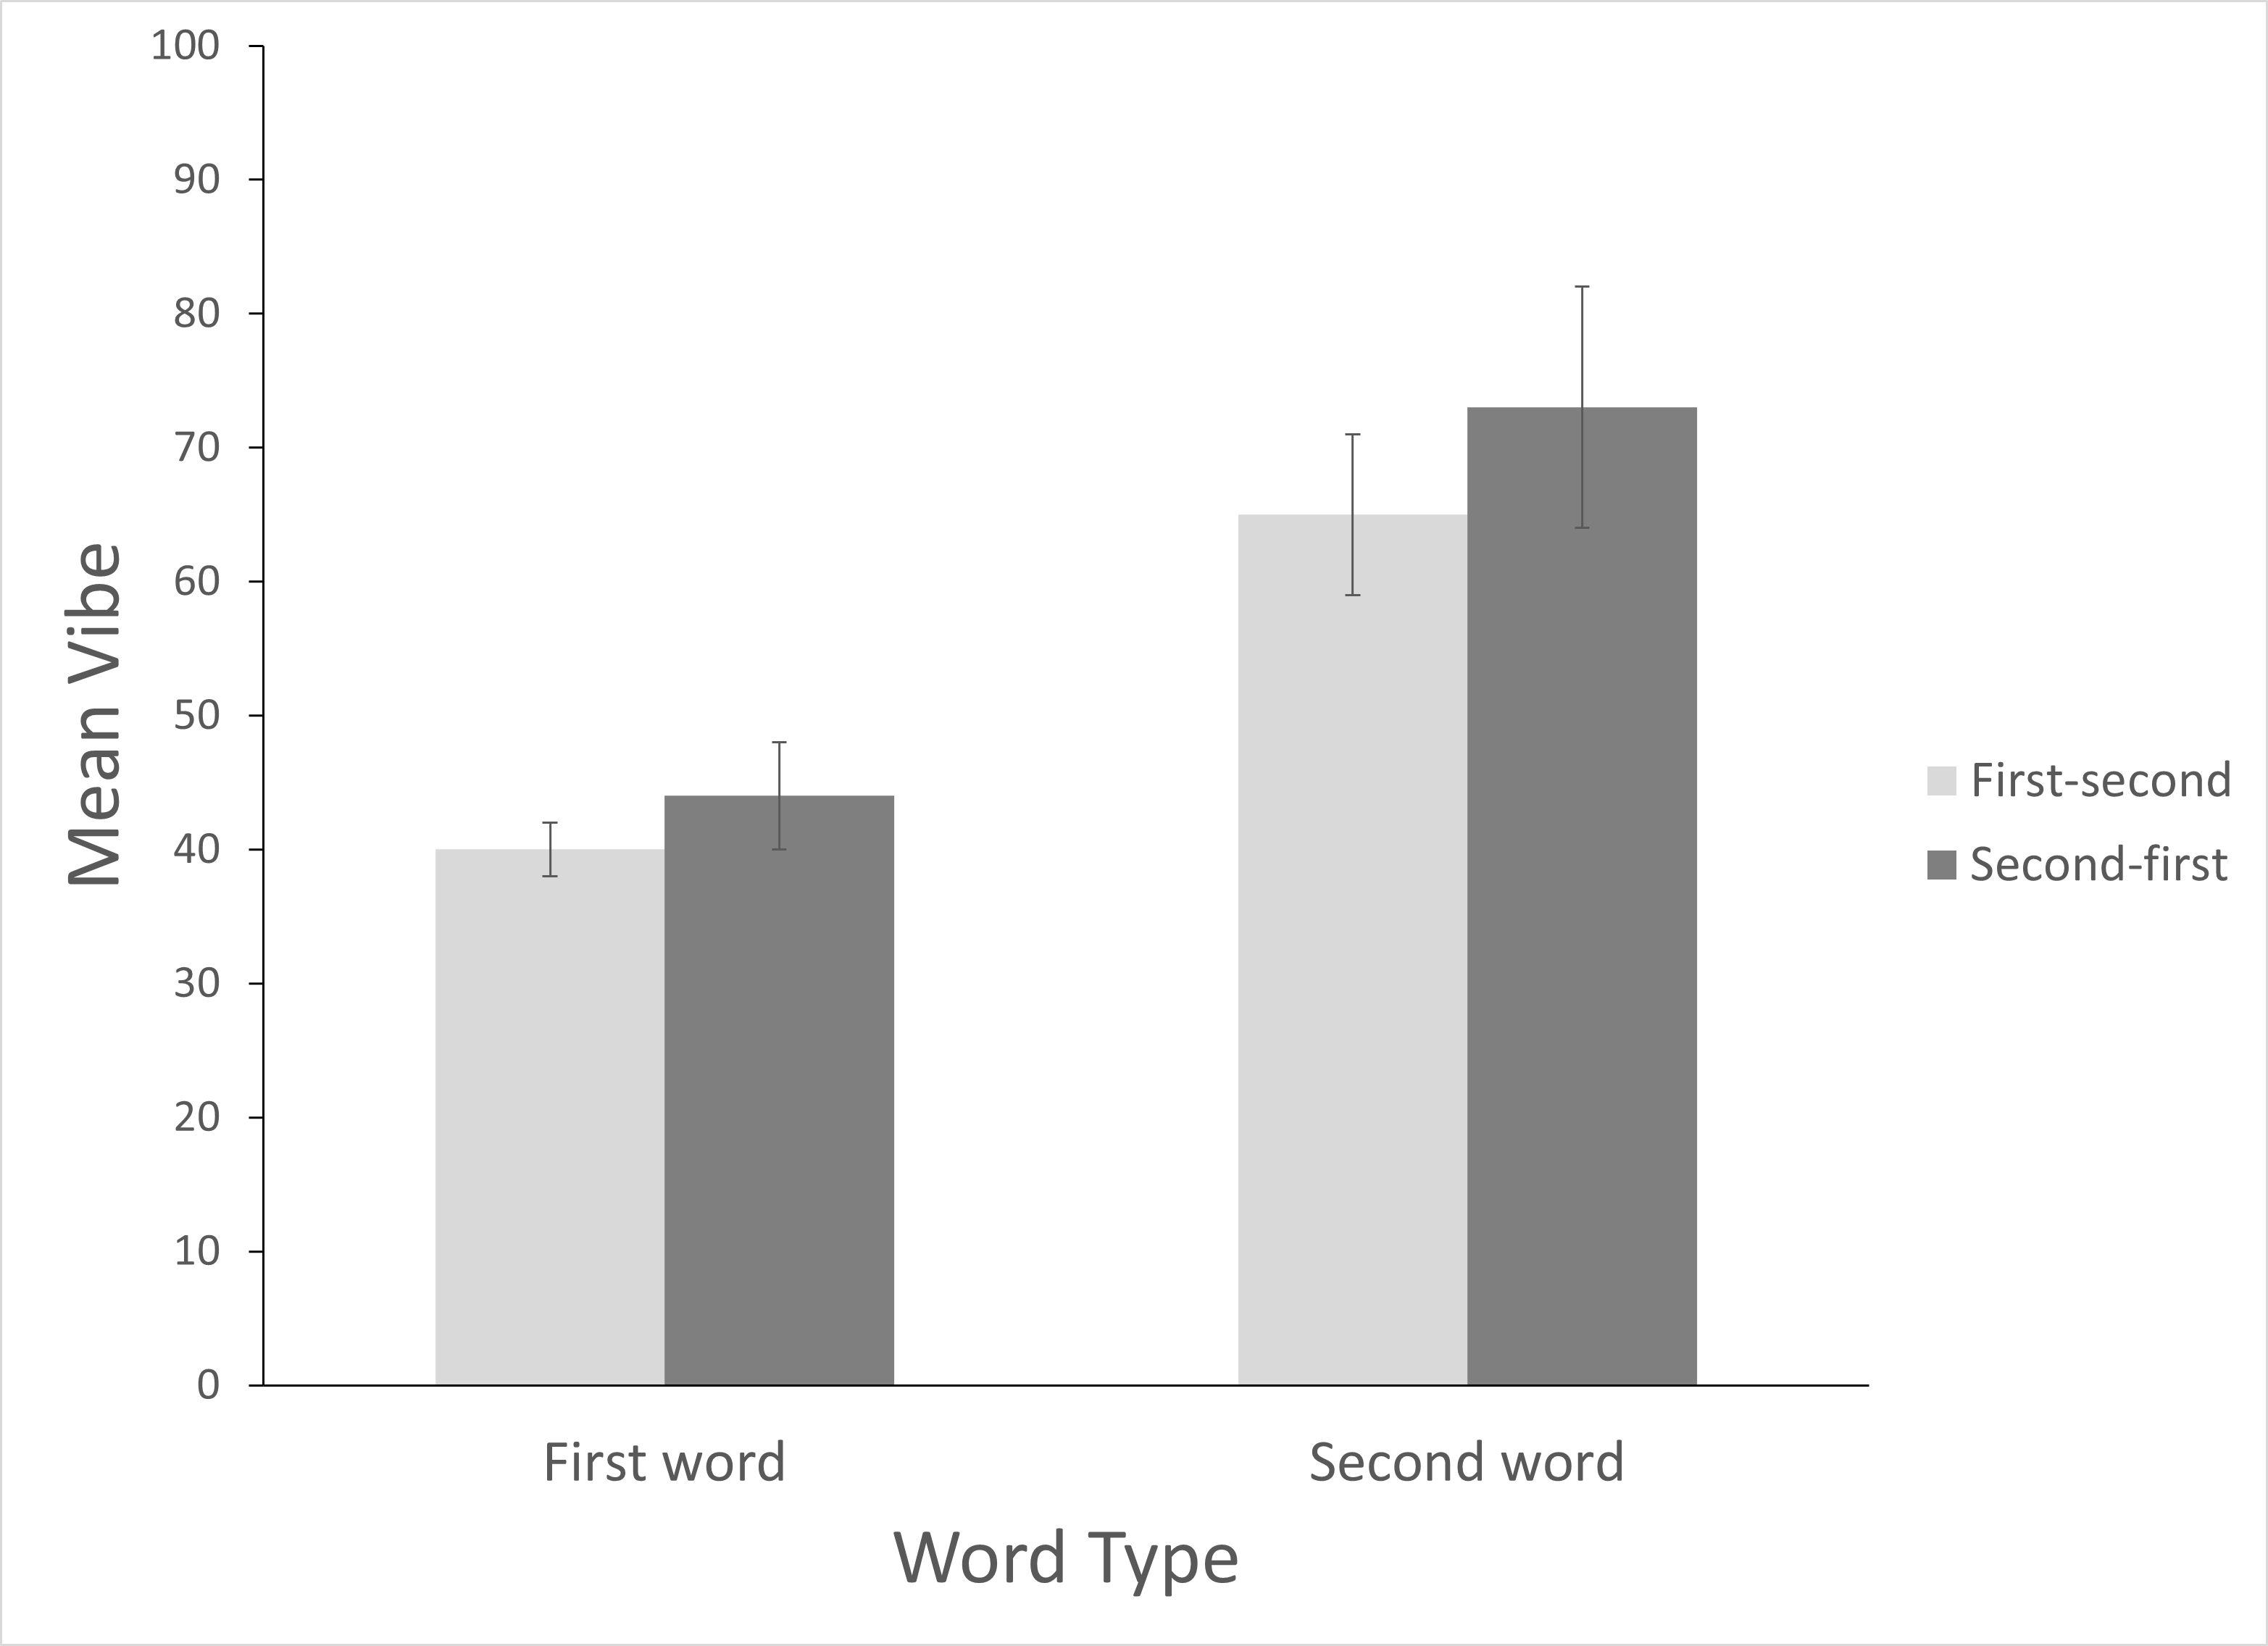
\includegraphics[width=0.75\linewidth]{sampleFig.png} % This is setting the figure to be .75x the width of the line. This can go all the way from 0.1 to 1 (and beyond, but then you're outside the page).
    \caption{The mean vibes for each word type and counterbalanced condition order. Error bars represent one standard error of the mean.}
    \label{fig:OverallEffect}
\end{figure}

Figure~\ref{fig:OverallEffect} shows the means and standard errors for the four experimental groups. As shown, the mean vibes for the second word ($M = $ 69, $SE = $ 7.5) were greater than the first word ($M = $ 42, $SE = $ 3), but roughly equivalent between presentation order conditions. Another fun little \LaTeX{} thing here: your instructor may explicitly want you to use $M$, but one of \LaTeX{}'s strengths is the easy of ``math mode'' (i.e., everything enclosed by the dollar signs). %In math mode, you can easily throw in Greek characters. So you \textit{could} instead present the descriptive statistics as ($\mu = $ 42). Oooh. Shiny. Although that seems to make Overleaf work extra hard, so I keep seeing a message encouraging upgrading to a paid plan, so I've commented this part out.

\subsection{Inferential Statistics}

This is where you start to do the actual statistical analysis. We generally tell students not to \textit{interpret} what the results mean until the discussion, but pay attention when reading journal articles - realistically a bit of interpretation does tend to happen at this point in published works.

A benefit of using \LaTeX{} is the ease in adding in macros to simplify your life. A common place I rolled these out in my dissertation were to make the formatting of all the analyses correct without a lot of work. I will include a couple example macros in the editor-side now, then use them in text. But, \textbf{another pro tip:} if you are going to deploy these macros, I would get in the habit of putting them up in the preamble so they are easier to find. Also, if you really get on board the \LaTeX{} train (which you should), you can recycle the preamble between projects, so those macros will also come along for the ride.

% A macro will have this format \newcommand{macroNameYoullUseToCallIt}[Number of inputs]{What the macro does} 
% The #s indicate where information will be slotted in when the macro is used
% The dollar signs indicate "math mode" is being used. It's mandatory for some functionality (like super/subscripts) or accessing the Greek alphabet used in statistical reporting.
% These macros are including the amount of info we expected from students when I was TAing labs. You can fill them out further if more info is required - just make sure you update the number in the square brackets!
\newcommand{\ttestSig}[2]{$t$(#1) = #2, $p < .05$}
\newcommand{\ttestInsig}[2]{$t$(#1) = #2, $p > .05$}
\newcommand{\anovaSig}[3]{$F$(#1,#2) = #3, $p < .05$}
\newcommand{\anovaInsig}[3]{$F$(#1,#2) = #3, $p > .05$}

Using the hypothetical experiment we have set up, let's say there was a significant interaction found between the word conditions (first versus second) and exposure order (first-second versus second-first), \anovaSig{11}{111}{4.20}. Pairwise comparisons indicate that this was driven by the words themselves, as there was a significant difference between the words, \ttestSig{111}{3.21}, but not for the exposure order, \ttestInsig{111}{.42}.

\section{Discussion}

As mentioned at the close of the Introduction, the Discussion starts out specific before building out to the broader picture. This will typically mean that the discussion starts with a reiteration of the Results, with more emphasis on interpretation. What differences were (or were not) found? Does this support your predictions, or have you failed to reject the null hypothesis? Statements of that nature.

With that done, you can work to tie your findings into the existing literature. Perhaps this result supports the work of \textcite{Contributor2023} but contradicts others \parencite[e.g.,][]{Sample2024}. %The extra square brackets here are telling LaTeX that the e.g., needs to be in front; it seems to assume otherwise that the e.g., belongs after the citation. Also note that I can have this comment here without breaking the paragraph. You need a double line break to separate paragraphs.
Why might this be the case? What similarities or differences exist between your experiment and the other works that could explain the differences? Or if the results are similar, what does this mean for the core theory (e.g., demonstrates it held up with different stimuli, or in a different context, or with different timing, etc.).

It is also important to work in potential limitations of your work. Frequently in undergrad cognitive lab reports, this will involve the sample size. It can be hard to reach significance when you have a sample size of 10. Other common limitations can be things like the stimuli didn't work out as you had hoped, the participants didn't understand the experiment directions (or were savvy to what you were testing which biased their data), or things you notice in running the experiment that you would do differently if you redid it in the future.

Finally, close things out by reiterating the brief version of your findings, what it means for the theory you were testing, and what it could mean for future research. Happy writing!



\printbibliography

\end{document}

%% 
%% Copyright (C) 2019 by Daniel A. Weiss <daniel.weiss.led at gmail.com>
%% 
%% This work may be distributed and/or modified under the
%% conditions of the LaTeX Project Public License (LPPL), either
%% version 1.3c of this license or (at your option) any later
%% version.  The latest version of this license is in the file:
%% 
%% http://www.latex-project.org/lppl.txt
%% 
%% Users may freely modify these files without permission, as long as the
%% copyright line and this statement are maintained intact.
%% 
%% This work is not endorsed by, affiliated with, or probably even known
%% by, the American Psychological Association.
%% 
%% This work is "maintained" (as per LPPL maintenance status) by
%% Daniel A. Weiss.
%% 
%% This work consists of the file  apa7.dtx
%% and the derived files           apa7.ins,
%%                                 apa7.cls,
%%                                 apa7.pdf,
%%                                 README,
%%                                 APA7american.txt,
%%                                 APA7british.txt,
%%                                 APA7dutch.txt,
%%                                 APA7english.txt,
%%                                 APA7german.txt,
%%                                 APA7ngerman.txt,
%%                                 APA7greek.txt,
%%                                 APA7czech.txt,
%%                                 APA7turkish.txt,
%%                                 APA7endfloat.cfg,
%%                                 Figure1.pdf,
%%                                 shortsample.tex,
%%                                 longsample.tex, and
%%                                 bibliography.bib.
%% 
%%
%%
%% This is file `./samples/shortsample.tex',
%% generated with the docstrip utility.
%%
%% The original source files were:
%%
%% apa7.dtx  (with options: `shortsample')
%% ----------------------------------------------------------------------
%% 
%% apa7 - A LaTeX class for formatting documents in compliance with the
%% American Psychological Association's Publication Manual, 7th edition
%% 
%% Copyright (C) 2019 by Daniel A. Weiss <daniel.weiss.led at gmail.com>
%% 
%% This work may be distributed and/or modified under the
%% conditions of the LaTeX Project Public License (LPPL), either
%% version 1.3c of this license or (at your option) any later
%% version.  The latest version of this license is in the file:
%% 
%% http://www.latex-project.org/lppl.txt
%% 
%% Users may freely modify these files without permission, as long as the
%% copyright line and this statement are maintained intact.
%% 
%% This work is not endorsed by, affiliated with, or probably even known
%% by, the American Psychological Association.
%% 
%% ----------------------------------------------------------------------